
\documentclass[preprint,12pt]{elsarticle}

\usepackage[spanish]{babel}
\usepackage{amssymb}
\usepackage{graphicx}
\usepackage{lineno}
\usepackage[utf8]{inputenc}
\usepackage{url}
\usepackage{natbib}

\begin{document}
	
	\begin{frontmatter}

		\title{\huge SQL: 2008  Estándar ISO / IEC 9075: 2008 de 2008}
		
		\author{Robles flores , Antnony Richard              (2016056192)}
		
		\address{Tacna, Perú}
		
		\begin{abstract}
			%% Text of abstract
ISO/IEC 9075 defines the SQL language. The scope of the SQL language is the definition of data structure and the operations on data stored in that structure. ISO/IEC 9075-1:2008, ISO/IEC 9075-2:2008 and ISO/IEC 9075-11:2008 encompass the minimum requirements of the language. Other parts define extensions.

ISO/IEC 9075-1:2008 specifies the conceptual framework used in other parts of ISO/IEC 9075 to specify the grammar of SQL and the result of processing statements in that language by an SQL-implementation.
		\end{abstract}
\end{frontmatter}
%%
	%% Start line numbering here if you want
	%%
	%\linenumbers
	
	%% main text
	\section{Resumen}

ISO / IEC 9075 define el lenguaje SQL. El alcance del lenguaje SQL es la definición de la estructura de datos y las operaciones sobre los datos almacenados en esa estructura. ISO / IEC 9075-1: 2008, ISO / IEC 9075-2: 2008 e ISO / IEC 9075-11: 2008 abarcan los requisitos mínimos del idioma. Otras partes definen extensiones.

ISO / IEC 9075-1: 2008 especifica el marco conceptual utilizado en otras partes de ISO / IEC 9075 para especificar la gramática de SQL y el resultado del procesamiento de declaraciones en ese lenguaje mediante una implementación de SQL.


%%INTRODUCCION%%-------------------------------------------------------------------------------------------
\section{Introducción}
El estándar SQL:2008 se divide en varias partes, que abarcan el Framework, la Fundación, el SQL/CLI, SQL/PSM, SQL/MED, SQL/OLB, SQL/Schemata, SQL/JRT Using Java, y varias especificaciones relacionadas.

Propiedades añadidas:
\begin{itemize}
\item Sentencias MERGE y DIAGNOSTIC mejoradas,
\item sentencias TRUNCATE TABLE,
\item cláusulas WHEN y expresiones CASE,
\item INSTEAD OF database trigger
\item JOIN,
\item soporte para varias expresiones regulares XQuery y
mejores al nombrado de las columnas derivadas.
\end{itemize}
%%-------------------------------------------------------------------------------------------

%MARCO TEORICO-------------------------------------------------------------------------------------------
\section{Marco Teórico}

\subsection{Definición}
El SQL (Structured query language), lenguaje de consulta estructurado, es un lenguaje surgido de un proyecto de investigación de IBM para el acceso a bases de datos relacionales. Actualmente se ha convertido en un estándar  de lenguaje de bases de datos, y la mayoría de los sistemas de bases de datos lo soportan, desde sistemas para ordenadores personales, hasta grandes ordenadores.\cite{DWarehouse02}
\\
\\

\begin{figure}[htb]
				\begin{center}
					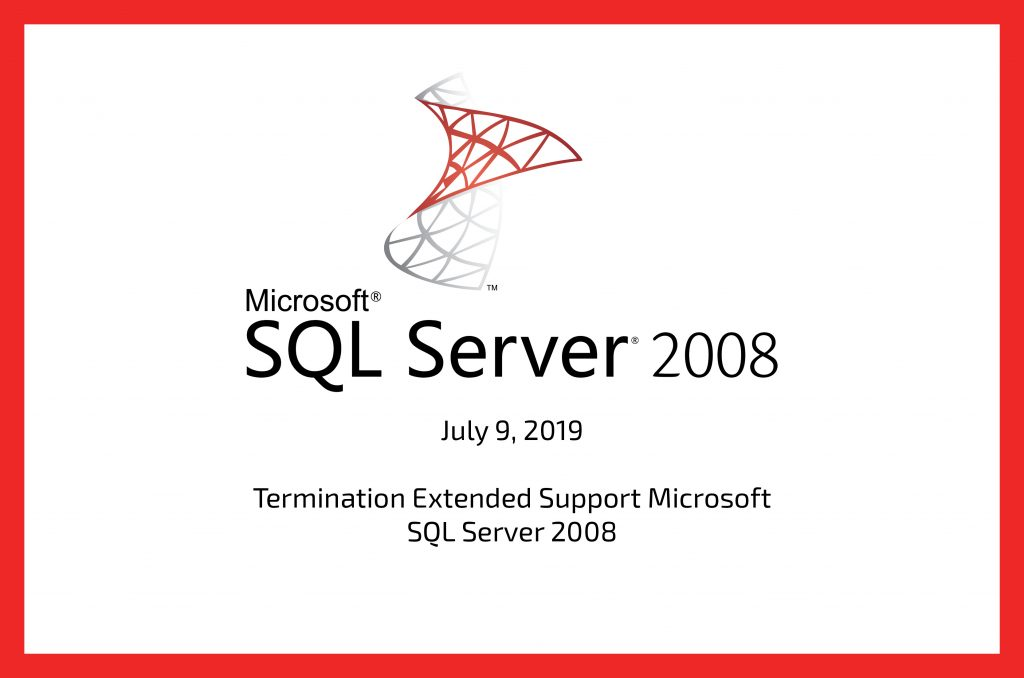
\includegraphics[width=9cm]{./IMAGENES/definicionsql}
				\end{center}
			\end{figure}

\subsection{Origen y eolución}
Los orígenes del SQL están ligados a los de las bases de datos relacionales. En 1970 E. F. Codd propone el modelo relacional y asociado a este un sublenguaje de acceso a los de datos basado en el cálculo de predicados. Basándose en estas ideas, los laboratorios de IBM definen el lenguaje sequele (Structured English Query Language) que más tarde sería ampliamente implementado por el sistemas de gestion de bases de datos (SGBD) experimental System R, desarrollado en 1977 también por IBM. Sin embargo, fue Oracle quien lo introdujo por primera vez en 1979 en un programa comercial.
\\
\\
El SEQUEL terminaría siendo el predecesor de SQL, siendo este una versión evolucionada del primero. El SQL pasa a ser el lenguaje por excelencia de los diversos sistemas de gestión de bases de datos relacionales surgidos en los años siguientes y es por fin estandarizado en 1986 por el ANSI, dando lugar a la primera versión estándar de este lenguaje, el "SQL-86" o "SQL1". Al año siguiente este estándar es también adoptado por la ISO.
Sin embargo, este primer estándar no cubre todas las necesidades de los desarrolladores e incluye funcionalidades de definición de almacenamiento que se consideró suprimirlas. Así que, en 1992, se lanzó un nuevo estándar ampliado y revisado del SQL llamado "SQL-92" o "SQL2".\cite{DWarehouse01}
\\
\\

\begin{figure}[htb]
				\begin{center}
					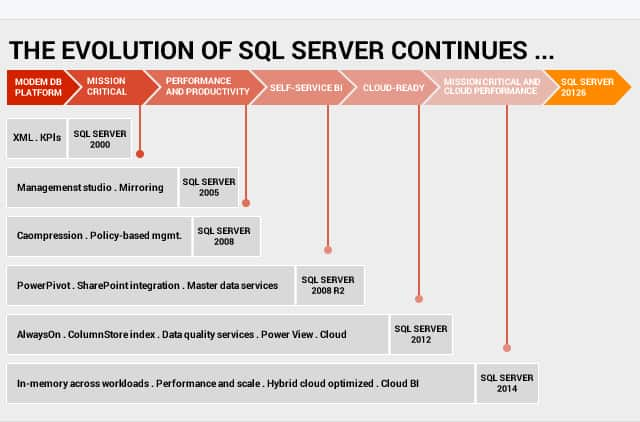
\includegraphics[width=10.5cm]{./IMAGENES/evolucion}
				\end{center}
			\end{figure}


\subsection{Características}
Muchas empresas usan servidores de Lenguaje de Consulta Estructurado (SQL por sus siglas en inglés) para manejar la colección de información de su empresa. Un servidor de bases de datos es una computadora que almacena los datos y le sirve la información al usuario cuando éste la pide. Existen varios tipos de sistemas de servidores de bases de datos, incluyendo los servidores SQL 2008 de Microsoft. Hay muchas ventajas al comprar e instalar un servidor SQL de Microsoft.
\\
\\
Soporta procedimientos almacenados. Incluye también un potente entorno gráfico de administración, que permite el uso de comandos DDL y DML gráficamente. Permite trabajar en modo cliente - servidor, donde la información y datos se alojan en el servidor y los terminales o clientes de la red sólo acceden a la información.
%%-------------------------------------------------------------------------------------------

%NOVEDADES-------------------------------------------------------------------------------------------
\section{Novedades lanzadas en SQL 2008}

\subsection{Definición}
Muchas de nuestras aplicaciones son aplicaciones conducidas o muy ligadas a los datos de una base de datos. Una de las tareas más «aburridas» para muchos desarrolladores es generar dicha capa de acceso a datos que les permita realizar las modificaciones de los datos. Además de frameworks como el Entity Framework en esta R2 CTP aparece el concepto de DAC (Data-tier application). SQL Server Management Studio proveerá de una forma sencilla de extraer directamente a partir de una base de datos que, Visual Studio de por medio, podrá ser enlazarda con nuestra aplicación como si un componente más de ésta se tratara. De esta forma podemos gestionar cambios en la base de datos junto a su actualización correspondiente en las aplicaciones con un simple instalable que corresponderá con la nueva versión de la "capa de acceso a la base de datos".
\\
\\

\subsection{SQL Server Utility}
En SQL Server 2008 se ha hecho un importante esfuerzo en centralizar y en permitir manejar un conjunto alto de instancias y servidores de forma centralizada y sencilla. Con la SQL Server Utility conseguimos tener una utilidad específica para la gestión del rendimiento y la configuración de éstas de forma unificada. Por supuesto nuevos informes se añadirán (tipo Dashboard) para poder mostrar toda esta información de forma gráfica. Creemos que esta utilidad tendrá un amplio uso entre administradores de granjas de servidores SQL Server, entornos virtualizados, etc.
\\
\\

\begin{figure}[htb]
				\begin{center}
					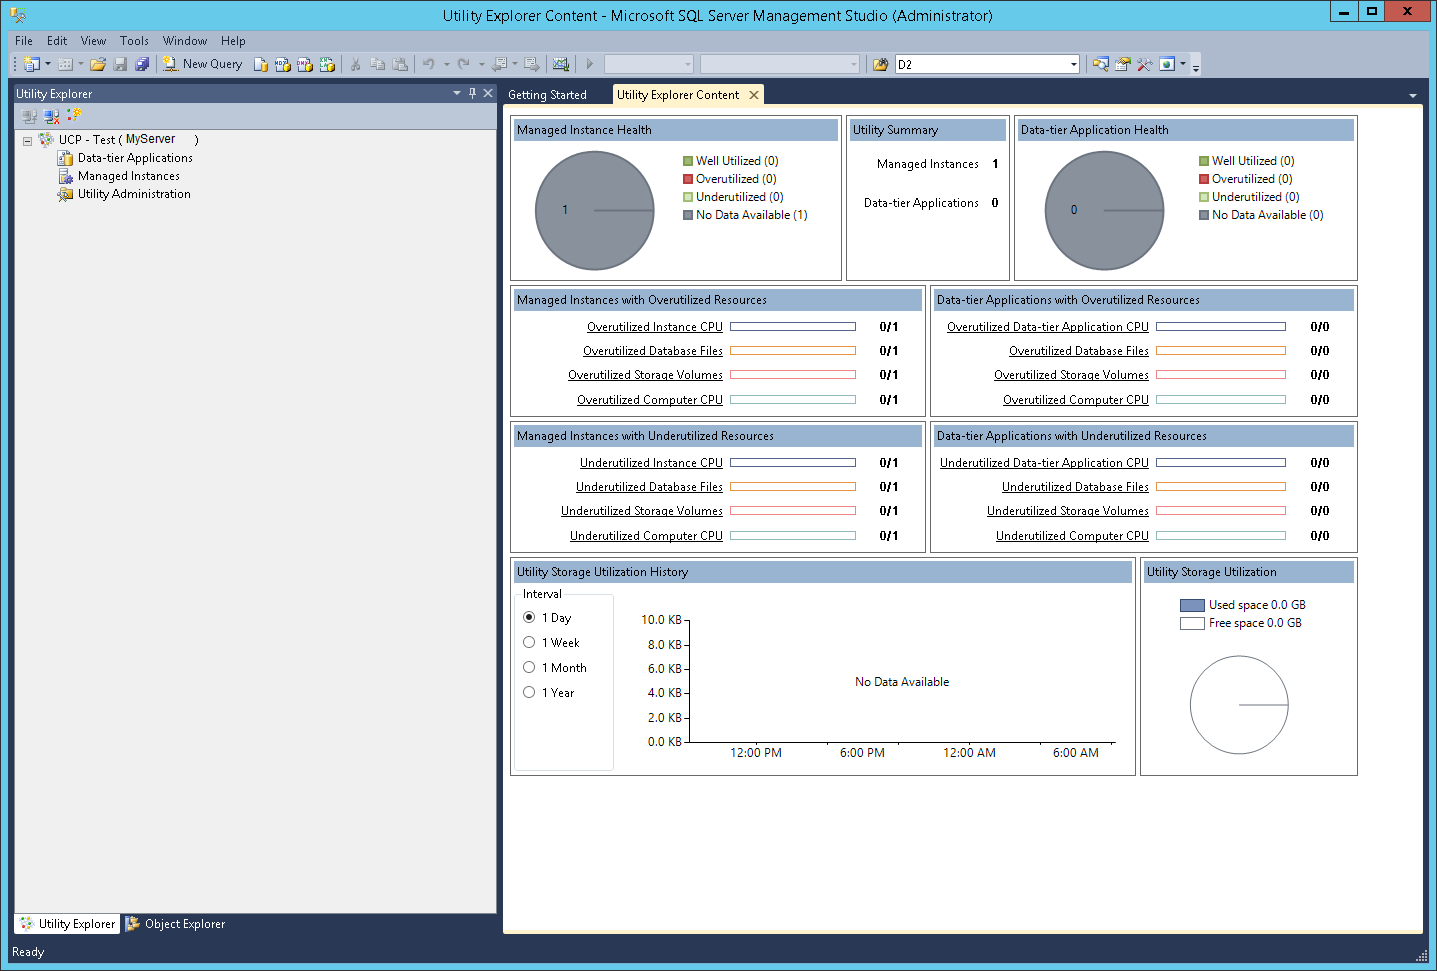
\includegraphics[width=10.5cm]{./IMAGENES/SQLServeUtility}
				\end{center}
			\end{figure}


\subsection{Compresión Unicode}
Con la cada vez mayor cantidad de cores por socket se llegaba a la situación de tener algunos servidores grandes con 96 procesadores de los cuales únicamente 64 podían ser utilizados por SQL Server 2008. Con la nueva revisión R2 ganamos «margen» hasta 512 CPUs por lo que, por ahora, no tendremos problemas para explotar al máximo todo el potencial de nuestros servidores.
\\
\\
\subsection{Soporte de hasta 512 CPUs}
En la revisión R2 se mejora el almacenamiento de los nchar(n) y nvarchar(n) utilizando la compresión SCSU (Standard Compression Scheme for Unicode). El grado de compresión obtenido rondará el 50\% para la mayoría de lenguajes que utilicen los caracteres más habituales como castellano o inglés J Una razón más para SIEMPRE utilizar UNICODE en nuestras cadenas de texto con contenido potencialmente multiidioma.

Finalmente recomendaros que quien se lance a instalar SQL Server 2008 R2 Side-by-side se lea bien las implicaciones de esto en los libros en pantalla pues bastantes componentes que serán compartidos entre ambas revisiones al no tratarse de una nueva versión al 100\% sino de una revisión de producto. Es por ello que prevemos muchas más actualizaciones inplace en estos escenarios antes que side-by-side.
\\

%%-------------------------------------------------------------------------------------------

%VENTAJAS-------------------------------------------------------------------------------------------
\section{Ventajas en SQL}

\subsection{Manos ayudantes}	
Un ventaja de instalar un sistema de servidores SQL es que estás uniendo una comunidad de servidores de SQL de Microsoft. En el 2008, el 20 por ciento del mercado de bases de datos pertenecían a los sistemas de servidores de SQL de Microsoft, según IDC, una firma independiente de investigación de mercado.
\\
\\
 IDC predice que un fuerte crecimiento continuará en la empresa. Encontrarás a muchos colegas en todo el mundo dispuestos a discutir problemas y soluciones en los grupos de usuarios de SQL, sitios web, sesiones de entrenamiento, listas de correos electrónicos y otros medios. 
\\
\\
Además, Microsoft tiene sus propias sesiones de entrenamiento y centro de soluciones disponible las 24 horas del día, los siete días de la semana. Microsoft ofrece soporte de sus productos y lanza actualizaciones y parches de sus sistemas regularmente para que tu sistema siga siendo funcional.\cite{DLake01}
\\

\subsection{Simple y lleno de características}	
Otro beneficio de los servidores SQL es la facilidad de usarlo y el mantenimiento. Ya que muchas personas están familiarizadas con los productos de Microsoft, usar la interfaz visual de un servidor SQL no es tan intimidatorio como otros programas. Existen muchas características que facilitan la creación de tu base de datos, como el Resource Governor (Gobernador de recursos). Según el escritor Don Schlichting de Database Journal, esta herramienta te permite vigilar a tus usuarios para que no usen todos los recursos de la base de datos con solicitudes. Al usar el servidor SQL, puedes decidir qué ancho de banda pueden tomar tus servidores y cuando se llegue a cierto nivel de uso, se puedan detener automáticamente los procesos que estén tomando demasiados recursos.\cite{DLake01}
\\
\subsection{Seguridad y estabilidad}
Muchos servidores SQL están están destinados a usarse en grandes grupos de datos y para manejar muchos usuarios. Cuando estás lidiando con varios usuarios y grandes cantidades de datos, necesitas un sistema que sea confiable (es decir, que no se caiga demasiado) y seguro (es decir, que se difícil de acceder sin autorización). En el lanzamiento del 2008 de SQL, una nueva característica es el Estudio de Desempeño. Esta colección de herramientas, dice Schlichting, pueden usarse para solucionar problemas, vigilar y configurar tu sistema para prevenir problemas que lleven a caídas del sistema.
\\
\\
 También, en SQL Server, tienes herramientas como la Administración Basada en Políticas que permite que los administradores de una base de datos definan políticas para los datos y para recibir alertas cuando las políticas sean violadas. También puedes codificar toda la base de datos, incluyendo tus datos y archivos de entrada, haciendo que tu servidor sea más seguro de ataques. Hay unas características de Administración de Contraseñas Externas que te permite ayudar a terceros certificados y codificar información en una sección separada, para que puedas manipular el procesamiento de tarjetas de crédito y seguir cumpliendo las leyes actuales de la industria de las tarjetas de crédito.  \cite{DLake01}	
%https://blogs.solidq.com/es/sql-server/novedades-sql-server-2008-r2/
%%-------------------------------------------------------------------------------------------

%DESVENTAJAS-------------------------------------------------------------------------------------------
\section{Desventajas en SQL}
MSSQL usa Address Windowing Extensión (AWE) para hacer el direccionamiento de 64 - bit. Esto le impide usar la administración dinámica de memoria y sólo le permite alojar un máximo de 64GB de memoria compartida. MSSQL no maneja compresión de datos (en SQL Server 2005 y 2000, solamente la versión 2008 Enterprise Edition incluye esta característica), por lo que ocupa mucho espacio en disco. MSSQL está atado a la plataforma del sistema operativo sobre la cual se instala una pésima implementación de los tipos de datos variables como varchar.\cite{DLake02}
%%-------------------------------------------------------------------------------------------

%CONCLUSIONES-------------------------------------------------------------------------------------------
\section{Conclusiones}

\subsection{Conclusión 1 : }	
Con sql nos permite ingresar comandos o sentencias de tal manera que podemos administrar o crear una base de datos.
Es la variedad de comandos que nos permiten generar datos desde la creación, modificasion o mantenimiento a las tablas las cuales también nos permiten recuperar datos o importarlos de siferentes maneras.

\subsection{Conclusión 2 : }	
Es difícil imaginar hoy en dia la concentración de información sin base de datos, las pequeñas o grandes industrias tienen como base su sistema informatico la construcción de base de datos con las que podemos tener una gran versatilidad incluso con los equipos myframe.
La seguridad en las bases de datos es muy importante debido a que garantiza la integridad física y la lógica de los datos de información.

%%-------------------------------------------------------------------------------------------

%%
	
	%%
	%\linenumbers
	
	%% main text

	
	\newpage
	
	\bibliographystyle{apalike} 	%ESTILO
	\bibliography{BIBLIOGRAFIA}	 
\citep{DLake01}  
\citep{DLake02}  
\citep{DWarehouse01}  
\citep{DWarehouse02}   
	

\end{document}

